Cette section regroupe les vues architecturales haute fidélité du système \gls{agentia} GraphRAG. Ces diagrammes illustrent la complexité des interactions entre les composants Dockerisés.

\section{Vue d'Ensemble du Système}

\begin{figure}[h]
    \centering
    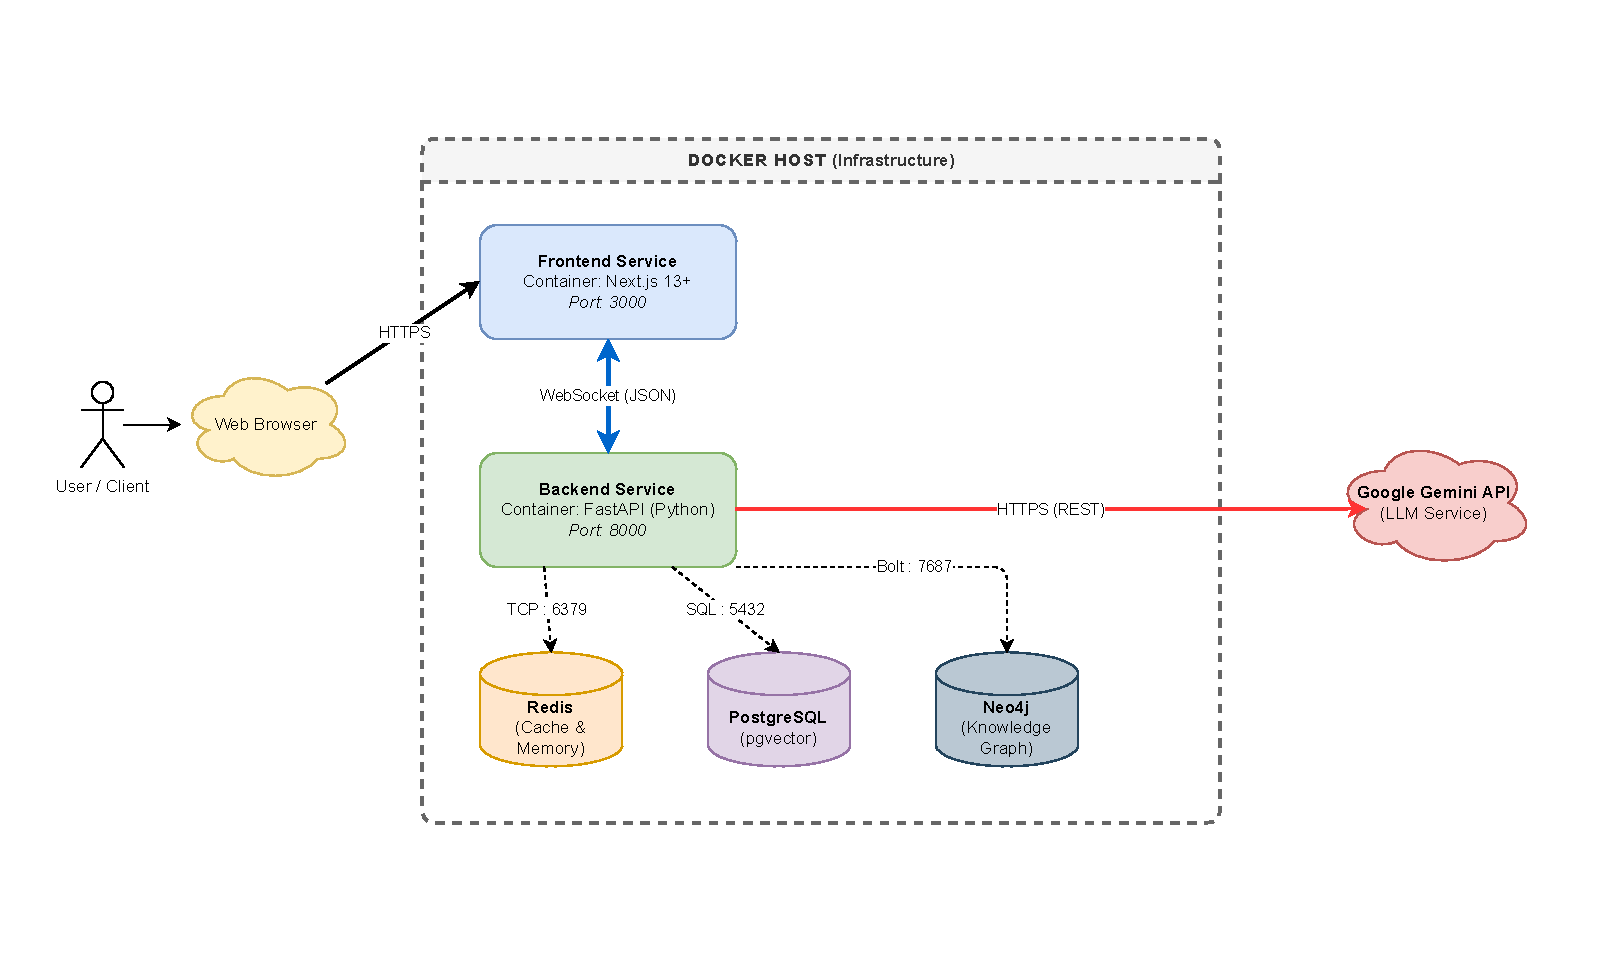
\includegraphics[width=1.0\textwidth]{docs/archi-globale.pdf} 
    \caption{\textbf{Architecture Micro-Services Hybride.} Vue globale montrant l'interaction entre le Frontend Next.js, le Backend FastAPI, et le cluster de bases de données (Redis, Neo4j, Postgres) piloté par un LLM Agnostique.}
    \label{fig:full_arch}
\end{figure}

\newpage

\section{Modélisation de la Connaissance (Ontologie)}

\begin{figure}[h]
    \centering
    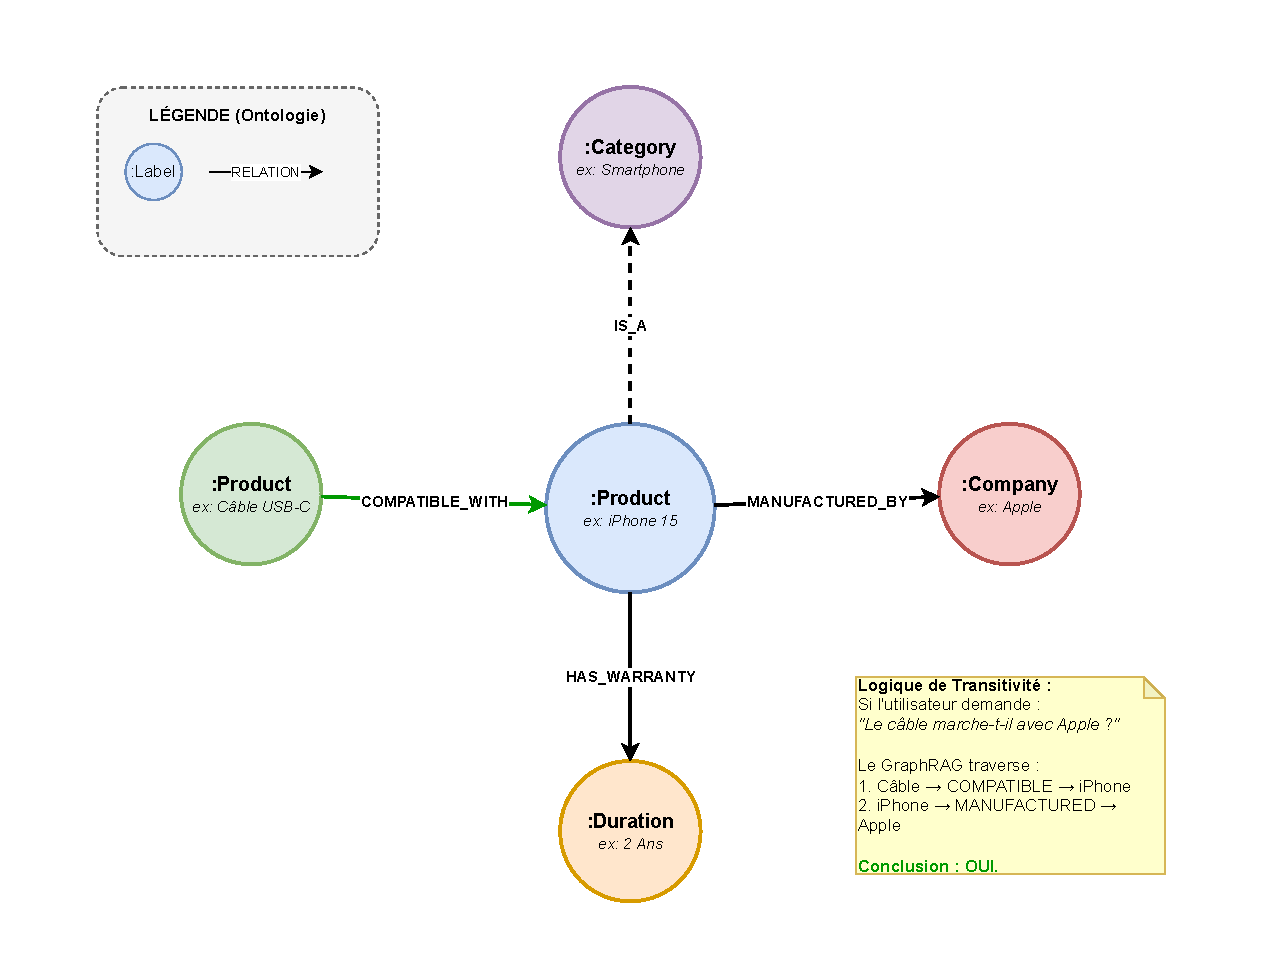
\includegraphics[width=0.85\textwidth]{docs/schema_graphe_metamodel.pdf}
    \caption{\textbf{Metamodel du GraphRAG.} Structure des nœuds et relations dans Neo4j permettant le raisonnement par transitivité (Compatibilité, Garantie).}
    \label{fig:ontology}
\end{figure}

\newpage

\section{Chronologie des Échanges}

\begin{figure}[h]
    \centering
    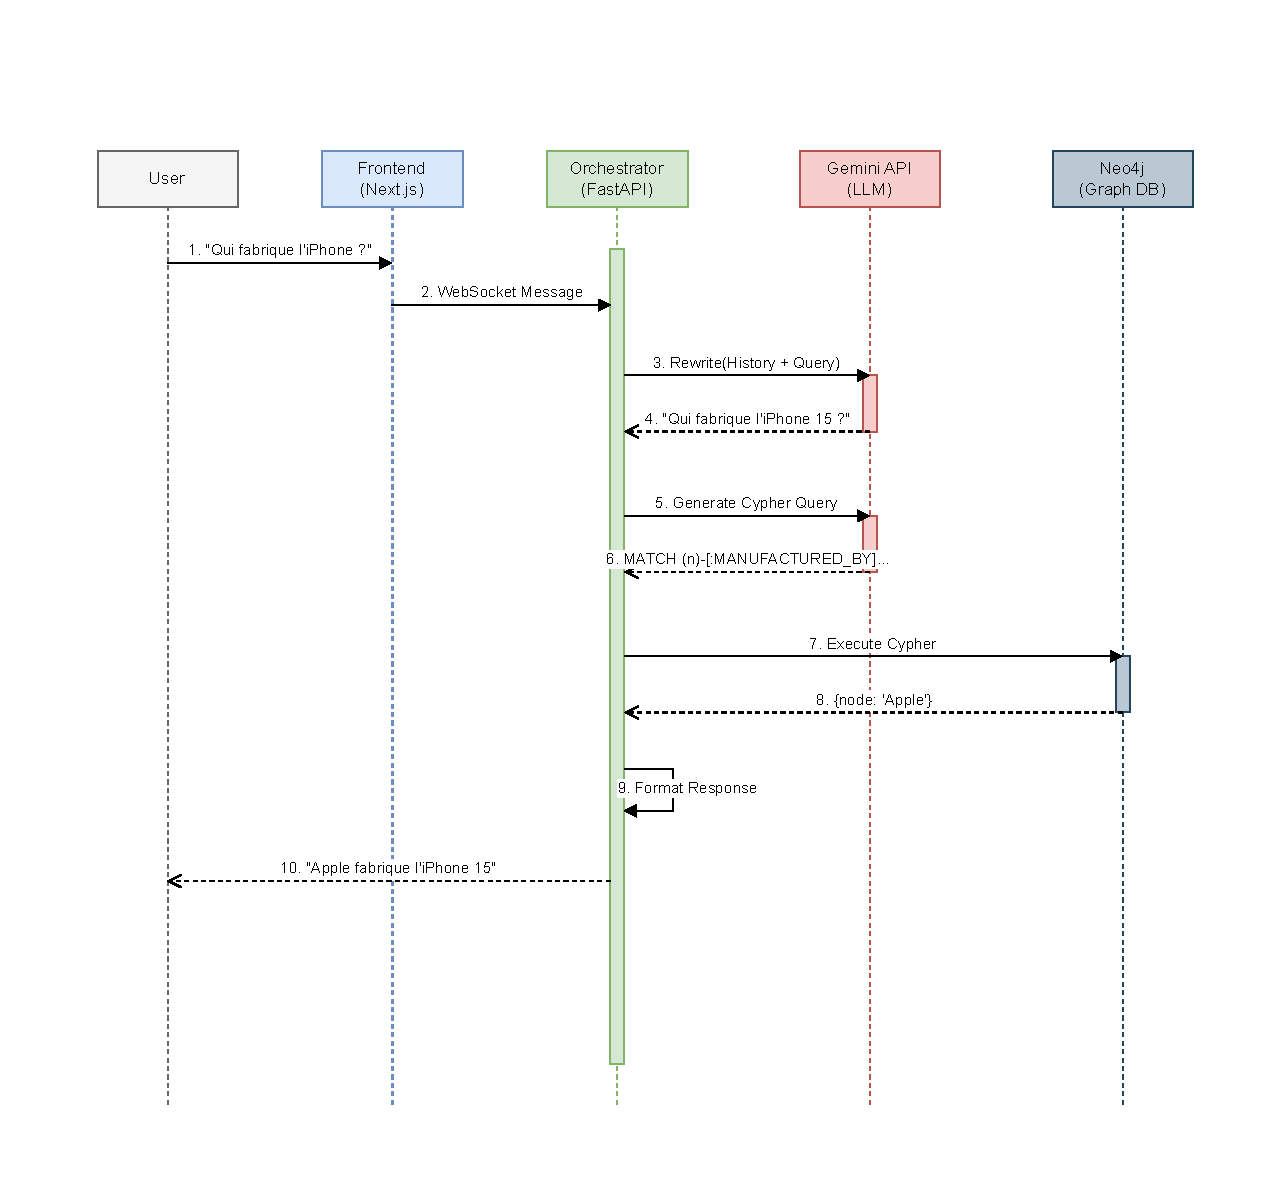
\includegraphics[width=1.0\textwidth]{docs/diagramme_sequence_message.pdf}
    \caption{\textbf{Diagramme de Séquence.} Flux détaillé d'un message utilisateur, montrant l'étape cruciale de "Contextual Rephrasing" avant l'interrogation de la base de données.}
    \label{fig:sequence}
\end{figure}

\newpage

\section{Pipeline d'Ingestion (ETL)}

\begin{figure}[h]
    \centering
    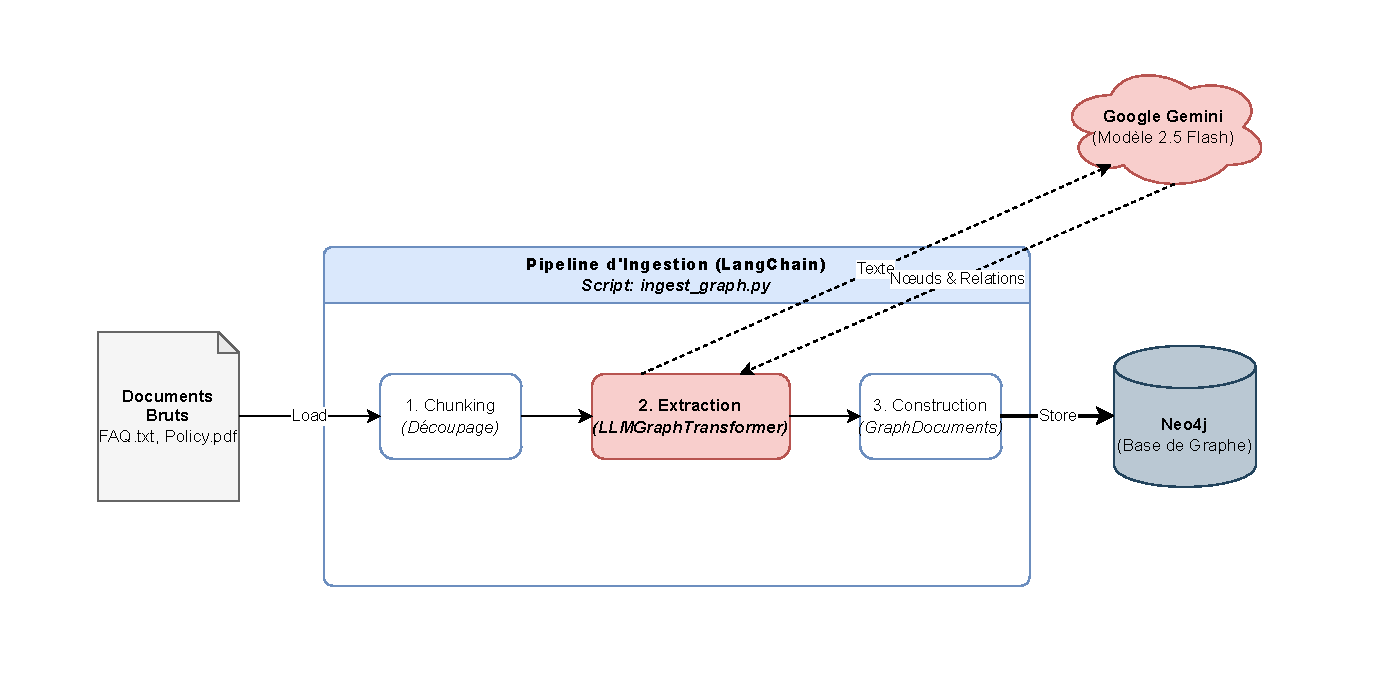
\includegraphics[width=1.0\textwidth]{docs/pipeline_etl.pdf}
    \caption{\textbf{Processus d'Ingestion Automatisé.} Transformation des documents non structurés en graphe structuré via l'utilisation d'un LLM comme extracteur d'entités.}
    \label{fig:etl}
\end{figure}


\newpage

\section{Logique Décisionnelle (Le Cerveau)}

\begin{figure}[h]
    \centering
    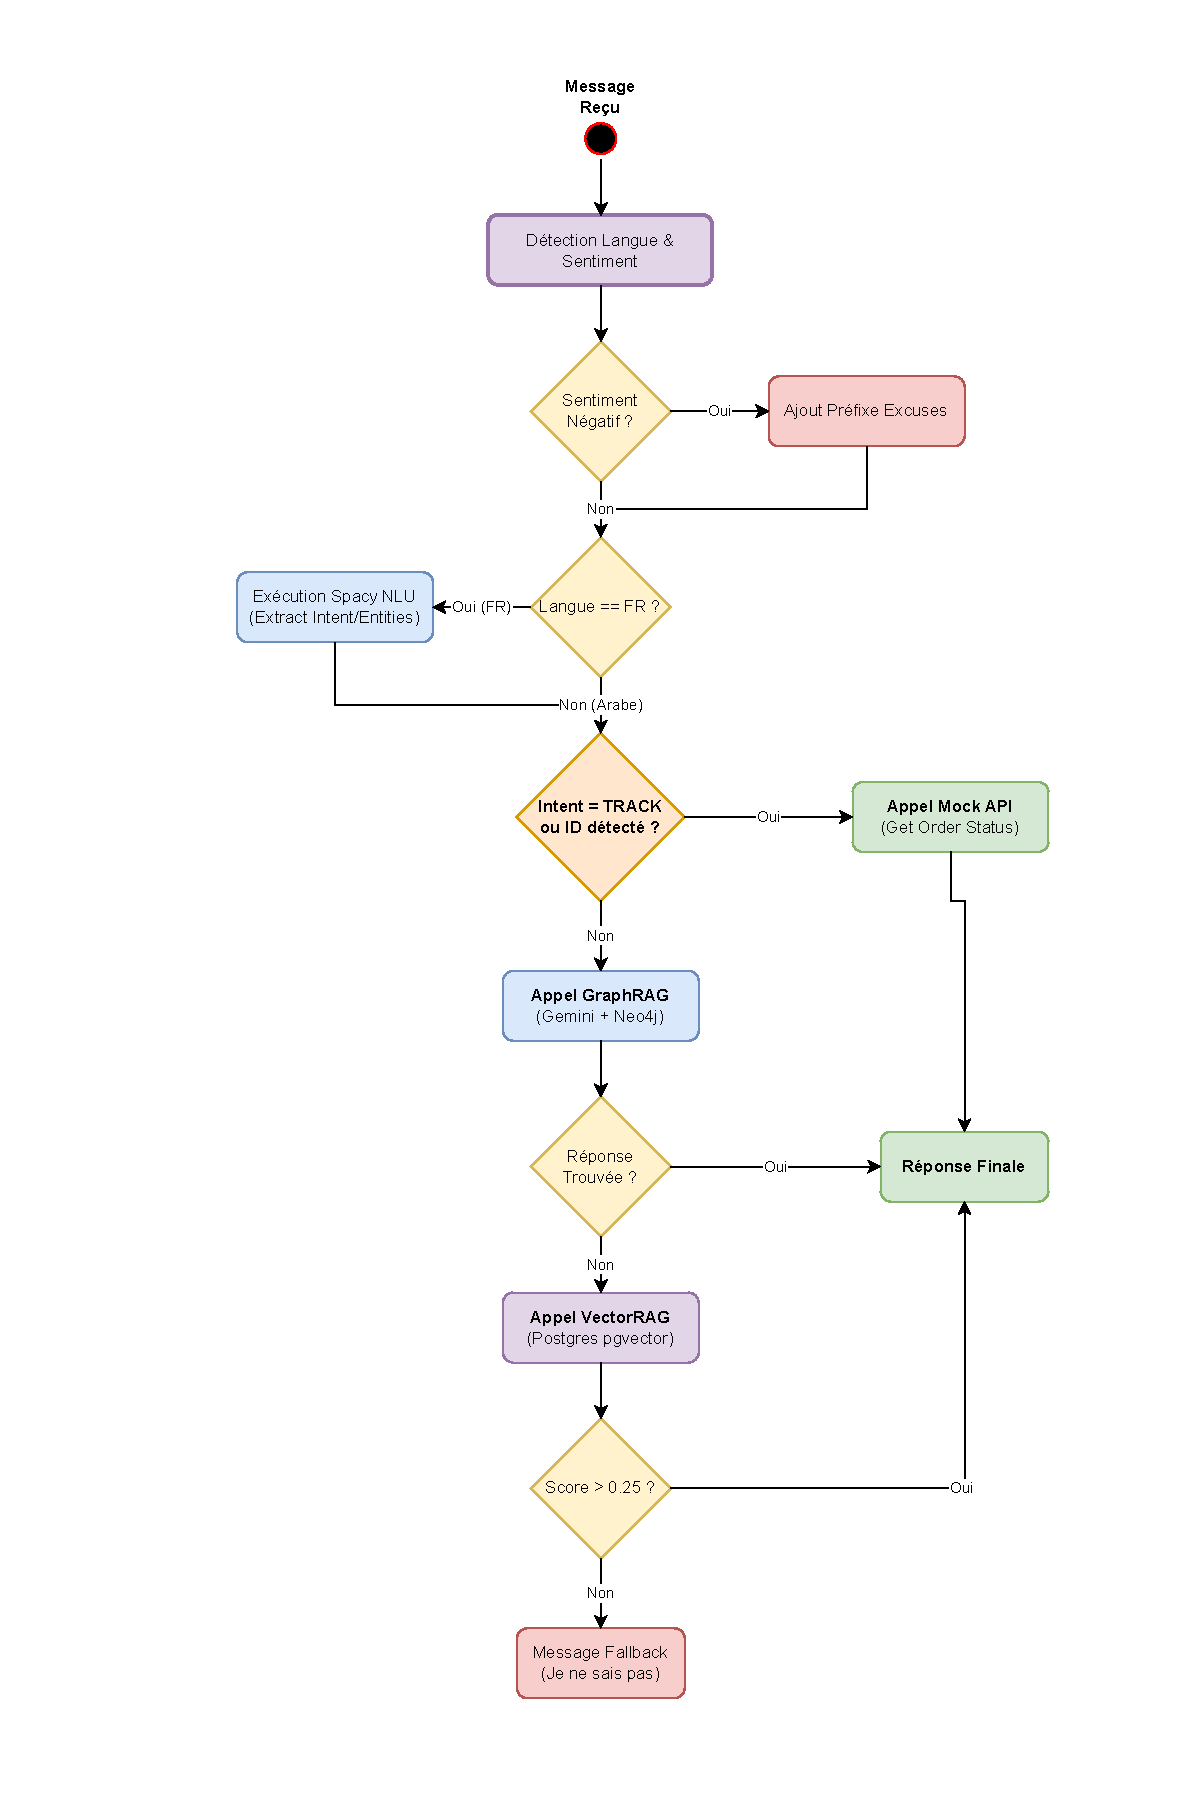
\includegraphics[width=0.55\textwidth]{docs/diagramme_activite_orchestrateur.pdf}
    \caption{\textbf{Algorithme de l'Orchestrateur.} Organigramme détaillant la stratégie de cascade : Détection $\rightarrow$ Transactionnel $\rightarrow$ GraphRAG $\rightarrow$ VectorRAG.}
    \label{fig:activity_flow}
\end{figure}

\newpage

\section{Dashboard des logs de l'admin}

\begin{figure}[h]
    \centering
    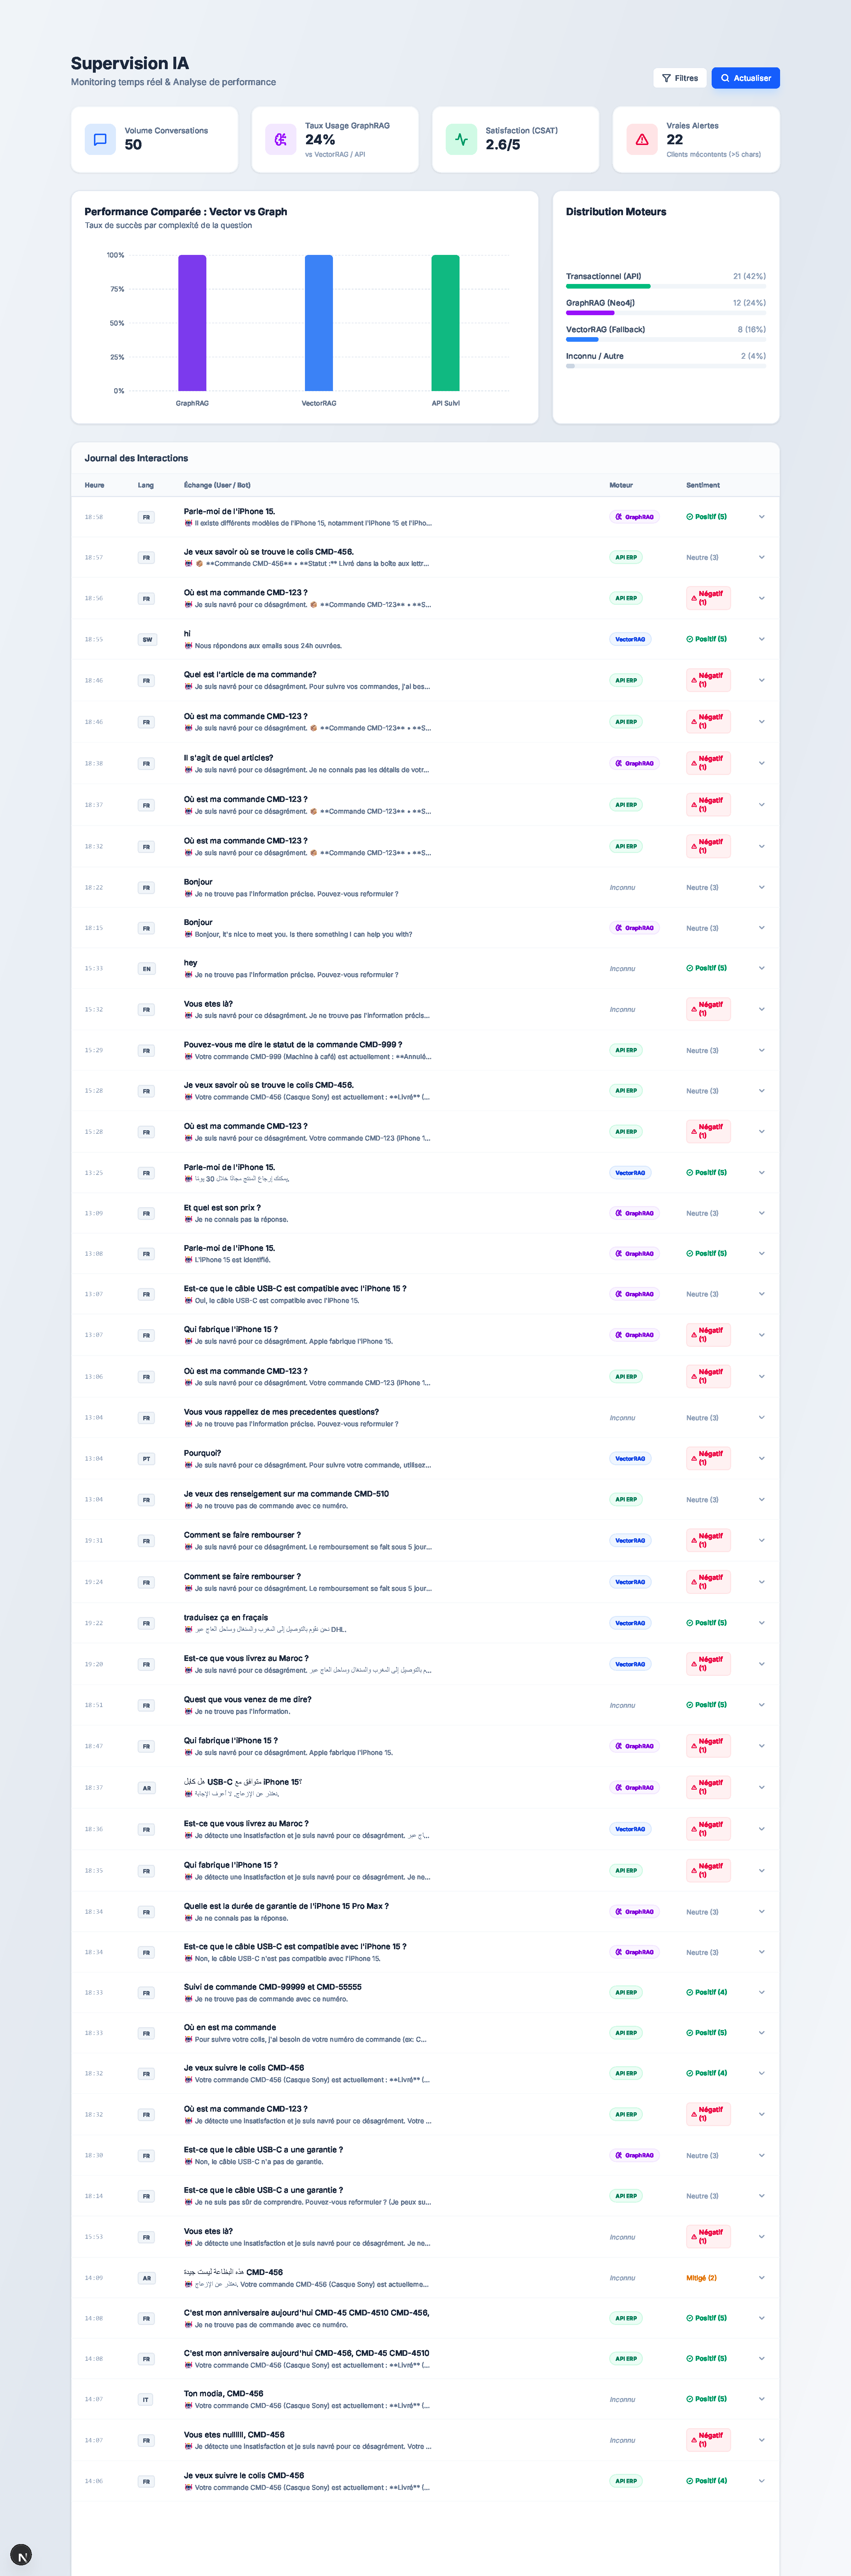
\includegraphics[width=1.0\textwidth]{docs/dashboard.pdf}
    \caption{\textbf{Le dashboard qui permet à l'admin de faire du monitoring.}}
    \label{fig:etl}
\end{figure}